\begin{frame}[fragile]{Visualização da construção do vetor $lcp$}

    \begin{figure}
        \centering

        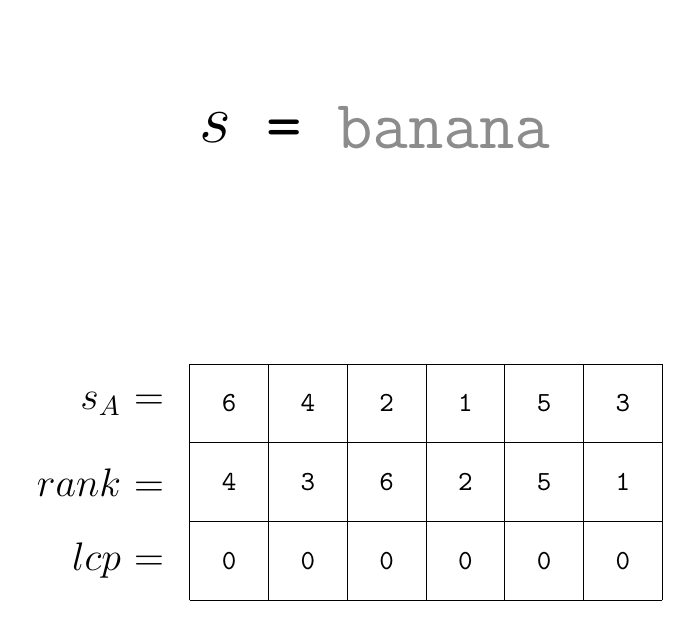
\begin{tikzpicture}
            \node[anchor=west] at (0, 5) { \Huge $s$ };
            \node[anchor=west] at (0.85, 5) { \Huge \texttt{= }\textcolor{gray!90}{\texttt{banana}} };
            \draw[opacity=0,<-] (2, 5.5) -- (2, 5.8) node[anchor=south] { $i$ };
            \draw[opacity=0,<-] (2.5, 4.5) -- (2.5, 4.2) node[anchor=north] { $j$ };

            \node[anchor=east] at (-0.2, 1.5) { \Large $s_A$ = };
            \draw (0, 1) grid (6, 2);
            \node[anchor=east] at (-0.2, 0.5) { \Large $rank$ = };
            \draw (0, 0) grid (6, 1);
            \node[anchor=east] at (-0.2, -0.5) { \Large $lcp$ = };
            \draw (0, -1) grid (6, 0);

            \node[opacity=0,anchor=west] at (-2.0, 3.0) { \Large $k = 0,$ };
            \node[opacity=0,anchor=west] at (1.0, 3.0) { \Large $i = 0,$ };
            \node[opacity=0,anchor=west] at (4.0, 3.0) { \Large $j = 0$ };

            \node at (0.5, 1.5) { \texttt{6} };
            \node at (1.5, 1.5) { \texttt{4} };
            \node at (2.5, 1.5) { \texttt{2} };
            \node at (3.5, 1.5) { \texttt{1} };
            \node at (4.5, 1.5) { \texttt{5} };
            \node at (5.5, 1.5) { \texttt{3} };

            \node at (0.5, 0.5) { {\texttt{4}} };
            \node at (1.5, 0.5) { {\texttt{3}} };
            \node at (2.5, 0.5) { {\texttt{6}} };
            \node at (3.5, 0.5) { {\texttt{2}} };
            \node at (4.5, 0.5) { {\texttt{5}} };
            \node at (5.5, 0.5) { {\texttt{1}} };

            \node at (0.5, -0.5) { {\texttt{0}} };
            \node at (1.5, -0.5) { {\texttt{0}} };
            \node at (2.5, -0.5) { {\texttt{0}} };
            \node at (3.5, -0.5) { {\texttt{0}} };
            \node at (4.5, -0.5) { {\texttt{0}} };
            \node at (5.5, -0.5) { {\texttt{0}} };


%            \node at (5.5, 0.5) { \textbf{\texttt{1}} };
        \end{tikzpicture}

    \end{figure}

\end{frame}

\begin{frame}[fragile]{Visualização da construção do vetor $lcp$}

    \begin{figure}
        \centering

        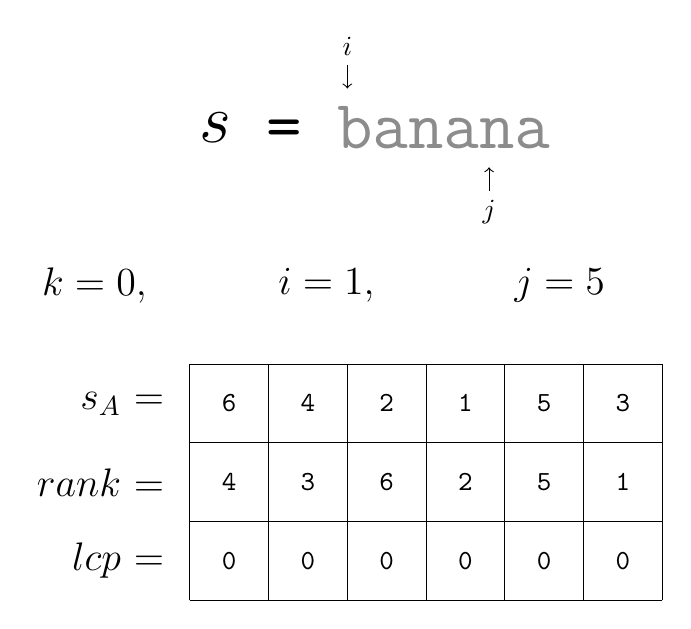
\begin{tikzpicture}
            \node[anchor=west] at (0, 5) { \Huge $s$ };
            \node[anchor=west] at (0.85, 5) { \Huge \texttt{= }\textcolor{gray!90}{\texttt{banana}} };
            \draw[opacity=1,<-] (2, 5.5) -- (2, 5.8) node[anchor=south] { $i$ };
            \draw[opacity=1,<-] (3.8, 4.5) -- (3.8, 4.2) node[anchor=north] { $j$ };

            \node[anchor=east] at (-0.2, 1.5) { \Large $s_A$ = };
            \draw (0, 1) grid (6, 2);
            \node[anchor=east] at (-0.2, 0.5) { \Large $rank$ = };
            \draw (0, 0) grid (6, 1);
            \node[anchor=east] at (-0.2, -0.5) { \Large $lcp$ = };
            \draw (0, -1) grid (6, 0);

            \node[opacity=1,anchor=west] at (-2.0, 3.0) { \Large $k = 0,$ };
            \node[opacity=1,anchor=west] at (1.0, 3.0) { \Large $i = 1,$ };
            \node[opacity=1,anchor=west] at (4.0, 3.0) { \Large $j = 5$ };

            \node at (0.5, 1.5) { \texttt{6} };
            \node at (1.5, 1.5) { \texttt{4} };
            \node at (2.5, 1.5) { \texttt{2} };
            \node at (3.5, 1.5) { \texttt{1} };
            \node at (4.5, 1.5) { \texttt{5} };
            \node at (5.5, 1.5) { \texttt{3} };

            \node at (0.5, 0.5) { {\texttt{4}} };
            \node at (1.5, 0.5) { {\texttt{3}} };
            \node at (2.5, 0.5) { {\texttt{6}} };
            \node at (3.5, 0.5) { {\texttt{2}} };
            \node at (4.5, 0.5) { {\texttt{5}} };
            \node at (5.5, 0.5) { {\texttt{1}} };

            \node at (0.5, -0.5) { {\texttt{0}} };
            \node at (1.5, -0.5) { {\texttt{0}} };
            \node at (2.5, -0.5) { {\texttt{0}} };
            \node at (3.5, -0.5) { \textbf{\texttt{0}} };
            \node at (4.5, -0.5) { {\texttt{0}} };
            \node at (5.5, -0.5) { {\texttt{0}} };


%            \node at (5.5, 0.5) { \textbf{\texttt{1}} };
        \end{tikzpicture}

    \end{figure}

\end{frame}

\begin{frame}[fragile]{Visualização da construção do vetor $lcp$}

    \begin{figure}
        \centering

        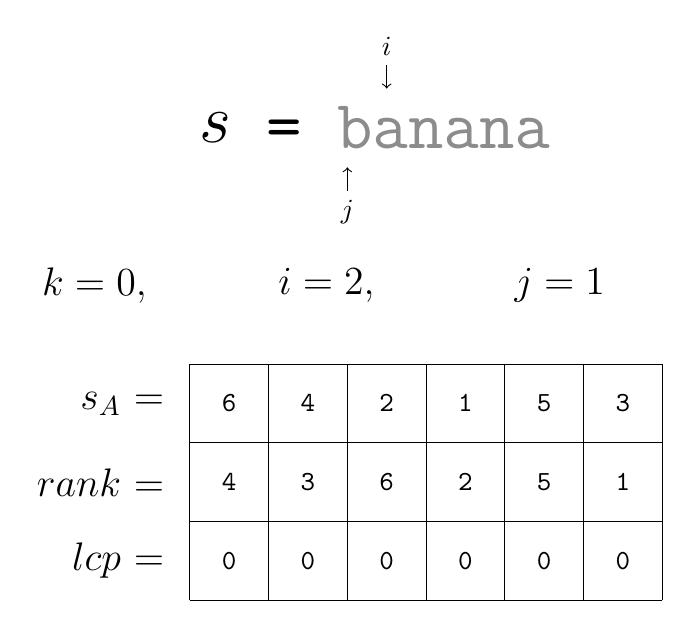
\begin{tikzpicture}
            \node[anchor=west] at (0, 5) { \Huge $s$ };
            \node[anchor=west] at (0.85, 5) { \Huge \texttt{= }\textcolor{gray!90}{\texttt{banana}} };
            \draw[opacity=1,<-] (2.5, 5.5) -- (2.5, 5.8) node[anchor=south] { $i$ };
            \draw[opacity=1,<-] (2.0, 4.5) -- (2.0, 4.2) node[anchor=north] { $j$ };

            \node[anchor=east] at (-0.2, 1.5) { \Large $s_A$ = };
            \draw (0, 1) grid (6, 2);
            \node[anchor=east] at (-0.2, 0.5) { \Large $rank$ = };
            \draw (0, 0) grid (6, 1);
            \node[anchor=east] at (-0.2, -0.5) { \Large $lcp$ = };
            \draw (0, -1) grid (6, 0);

            \node[opacity=1,anchor=west] at (-2.0, 3.0) { \Large $k = 0,$ };
            \node[opacity=1,anchor=west] at (1.0, 3.0) { \Large $i = 2,$ };
            \node[opacity=1,anchor=west] at (4.0, 3.0) { \Large $j = 1$ };

            \node at (0.5, 1.5) { \texttt{6} };
            \node at (1.5, 1.5) { \texttt{4} };
            \node at (2.5, 1.5) { \texttt{2} };
            \node at (3.5, 1.5) { \texttt{1} };
            \node at (4.5, 1.5) { \texttt{5} };
            \node at (5.5, 1.5) { \texttt{3} };

            \node at (0.5, 0.5) { {\texttt{4}} };
            \node at (1.5, 0.5) { {\texttt{3}} };
            \node at (2.5, 0.5) { {\texttt{6}} };
            \node at (3.5, 0.5) { {\texttt{2}} };
            \node at (4.5, 0.5) { {\texttt{5}} };
            \node at (5.5, 0.5) { {\texttt{1}} };

            \node at (0.5, -0.5) { {\texttt{0}} };
            \node at (1.5, -0.5) { {\texttt{0}} };
            \node at (2.5, -0.5) { \textbf{\texttt{0}} };
            \node at (3.5, -0.5) { {\texttt{0}} };
            \node at (4.5, -0.5) { {\texttt{0}} };
            \node at (5.5, -0.5) { {\texttt{0}} };


%            \node at (5.5, 0.5) { \textbf{\texttt{1}} };
        \end{tikzpicture}

    \end{figure}

\end{frame}

\begin{frame}[fragile]{Visualização da construção do vetor $lcp$}

    \begin{figure}
        \centering

        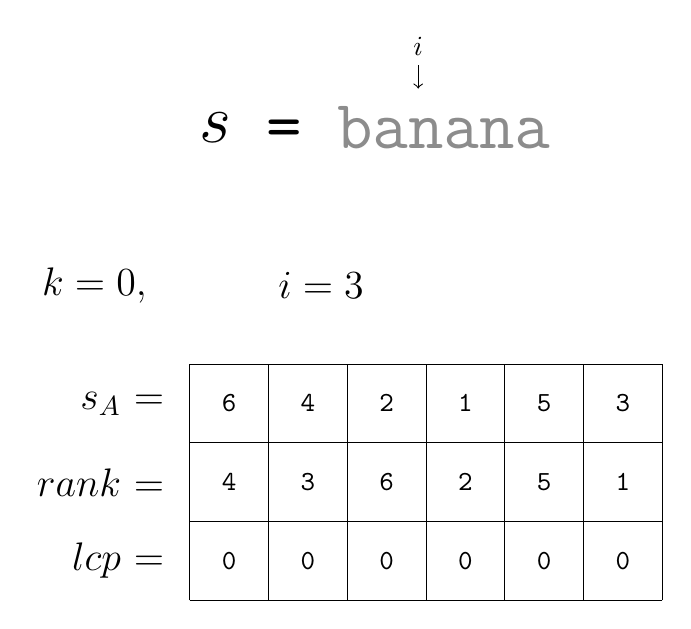
\begin{tikzpicture}
            \node[anchor=west] at (0, 5) { \Huge $s$ };
            \node[anchor=west] at (0.85, 5) { \Huge \texttt{= }\textcolor{gray!90}{\texttt{banana}} };
            \draw[opacity=1,<-] (2.9, 5.5) -- (2.9, 5.8) node[anchor=south] { $i$ };
            \draw[opacity=0,<-] (2.0, 4.5) -- (2.0, 4.2) node[anchor=north] { $j$ };

            \node[anchor=east] at (-0.2, 1.5) { \Large $s_A$ = };
            \draw (0, 1) grid (6, 2);
            \node[anchor=east] at (-0.2, 0.5) { \Large $rank$ = };
            \draw (0, 0) grid (6, 1);
            \node[anchor=east] at (-0.2, -0.5) { \Large $lcp$ = };
            \draw (0, -1) grid (6, 0);

            \node[opacity=1,anchor=west] at (-2.0, 3.0) { \Large $k = 0,$ };
            \node[opacity=1,anchor=west] at (1.0, 3.0) { \Large $i = 3$ };
            \node[opacity=0,anchor=west] at (4.0, 3.0) { \Large $j = 1$ };

            \node at (0.5, 1.5) { \texttt{6} };
            \node at (1.5, 1.5) { \texttt{4} };
            \node at (2.5, 1.5) { \texttt{2} };
            \node at (3.5, 1.5) { \texttt{1} };
            \node at (4.5, 1.5) { \texttt{5} };
            \node at (5.5, 1.5) { \texttt{3} };

            \node at (0.5, 0.5) { {\texttt{4}} };
            \node at (1.5, 0.5) { {\texttt{3}} };
            \node at (2.5, 0.5) { {\texttt{6}} };
            \node at (3.5, 0.5) { {\texttt{2}} };
            \node at (4.5, 0.5) { {\texttt{5}} };
            \node at (5.5, 0.5) { {\texttt{1}} };

            \node at (0.5, -0.5) { {\texttt{0}} };
            \node at (1.5, -0.5) { {\texttt{0}} };
            \node at (2.5, -0.5) { {\texttt{0}} };
            \node at (3.5, -0.5) { {\texttt{0}} };
            \node at (4.5, -0.5) { {\texttt{0}} };
            \node at (5.5, -0.5) { \textbf{\texttt{0}} };


%            \node at (5.5, 0.5) { \textbf{\texttt{1}} };
        \end{tikzpicture}

    \end{figure}

\end{frame}

\begin{frame}[fragile]{Visualização da construção do vetor $lcp$}

    \begin{figure}
        \centering

        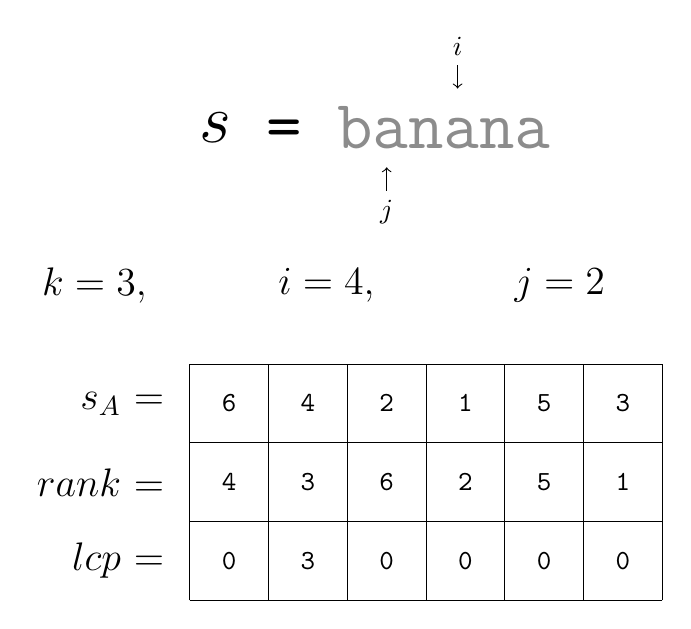
\begin{tikzpicture}
            \node[anchor=west] at (0, 5) { \Huge $s$ };
            \node[anchor=west] at (0.85, 5) { \Huge \texttt{= }\textcolor{gray!90}{\texttt{banana}} };
            \draw[opacity=1,<-] (3.4, 5.5) -- (3.4, 5.8) node[anchor=south] { $i$ };
            \draw[opacity=1,<-] (2.5, 4.5) -- (2.5, 4.2) node[anchor=north] { $j$ };

            \node[anchor=east] at (-0.2, 1.5) { \Large $s_A$ = };
            \draw (0, 1) grid (6, 2);
            \node[anchor=east] at (-0.2, 0.5) { \Large $rank$ = };
            \draw (0, 0) grid (6, 1);
            \node[anchor=east] at (-0.2, -0.5) { \Large $lcp$ = };
            \draw (0, -1) grid (6, 0);

            \node[opacity=1,anchor=west] at (-2.0, 3.0) { \Large $k = 3,$ };
            \node[opacity=1,anchor=west] at (1.0, 3.0) { \Large $i = 4,$ };
            \node[opacity=1,anchor=west] at (4.0, 3.0) { \Large $j = 2$ };

            \node at (0.5, 1.5) { \texttt{6} };
            \node at (1.5, 1.5) { \texttt{4} };
            \node at (2.5, 1.5) { \texttt{2} };
            \node at (3.5, 1.5) { \texttt{1} };
            \node at (4.5, 1.5) { \texttt{5} };
            \node at (5.5, 1.5) { \texttt{3} };

            \node at (0.5, 0.5) { {\texttt{4}} };
            \node at (1.5, 0.5) { {\texttt{3}} };
            \node at (2.5, 0.5) { {\texttt{6}} };
            \node at (3.5, 0.5) { {\texttt{2}} };
            \node at (4.5, 0.5) { {\texttt{5}} };
            \node at (5.5, 0.5) { {\texttt{1}} };

            \node at (0.5, -0.5) { {\texttt{0}} };
            \node at (1.5, -0.5) { \textbf{\texttt{3}} };
            \node at (2.5, -0.5) { {\texttt{0}} };
            \node at (3.5, -0.5) { {\texttt{0}} };
            \node at (4.5, -0.5) { {\texttt{0}} };
            \node at (5.5, -0.5) { {\texttt{0}} };


%            \node at (5.5, 0.5) { \textbf{\texttt{1}} };
        \end{tikzpicture}

    \end{figure}

\end{frame}

\begin{frame}[fragile]{Visualização da construção do vetor $lcp$}

    \begin{figure}
        \centering

        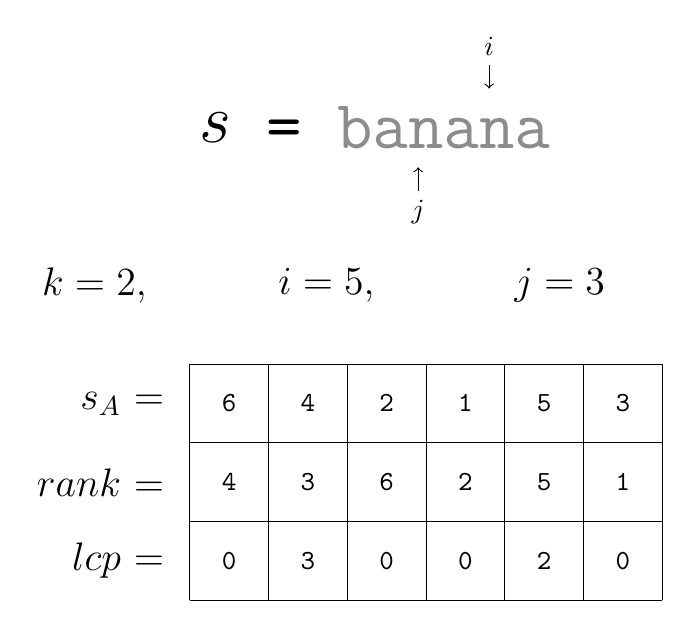
\begin{tikzpicture}
            \node[anchor=west] at (0, 5) { \Huge $s$ };
            \node[anchor=west] at (0.85, 5) { \Huge \texttt{= }\textcolor{gray!90}{\texttt{banana}} };
            \draw[opacity=1,<-] (3.8, 5.5) -- (3.8, 5.8) node[anchor=south] { $i$ };
            \draw[opacity=1,<-] (2.9, 4.5) -- (2.9, 4.2) node[anchor=north] { $j$ };

            \node[anchor=east] at (-0.2, 1.5) { \Large $s_A$ = };
            \draw (0, 1) grid (6, 2);
            \node[anchor=east] at (-0.2, 0.5) { \Large $rank$ = };
            \draw (0, 0) grid (6, 1);
            \node[anchor=east] at (-0.2, -0.5) { \Large $lcp$ = };
            \draw (0, -1) grid (6, 0);

            \node[opacity=1,anchor=west] at (-2.0, 3.0) { \Large $k = 2,$ };
            \node[opacity=1,anchor=west] at (1.0, 3.0) { \Large $i = 5,$ };
            \node[opacity=1,anchor=west] at (4.0, 3.0) { \Large $j = 3$ };

            \node at (0.5, 1.5) { \texttt{6} };
            \node at (1.5, 1.5) { \texttt{4} };
            \node at (2.5, 1.5) { \texttt{2} };
            \node at (3.5, 1.5) { \texttt{1} };
            \node at (4.5, 1.5) { \texttt{5} };
            \node at (5.5, 1.5) { \texttt{3} };

            \node at (0.5, 0.5) { {\texttt{4}} };
            \node at (1.5, 0.5) { {\texttt{3}} };
            \node at (2.5, 0.5) { {\texttt{6}} };
            \node at (3.5, 0.5) { {\texttt{2}} };
            \node at (4.5, 0.5) { {\texttt{5}} };
            \node at (5.5, 0.5) { {\texttt{1}} };

            \node at (0.5, -0.5) { {\texttt{0}} };
            \node at (1.5, -0.5) { {\texttt{3}} };
            \node at (2.5, -0.5) { {\texttt{0}} };
            \node at (3.5, -0.5) { {\texttt{0}} };
            \node at (4.5, -0.5) { \textbf{\texttt{2}} };
            \node at (5.5, -0.5) { {\texttt{0}} };


%            \node at (5.5, 0.5) { \textbf{\texttt{1}} };
        \end{tikzpicture}

    \end{figure}

\end{frame}

\begin{frame}[fragile]{Visualização da construção do vetor $lcp$}

    \begin{figure}
        \centering

        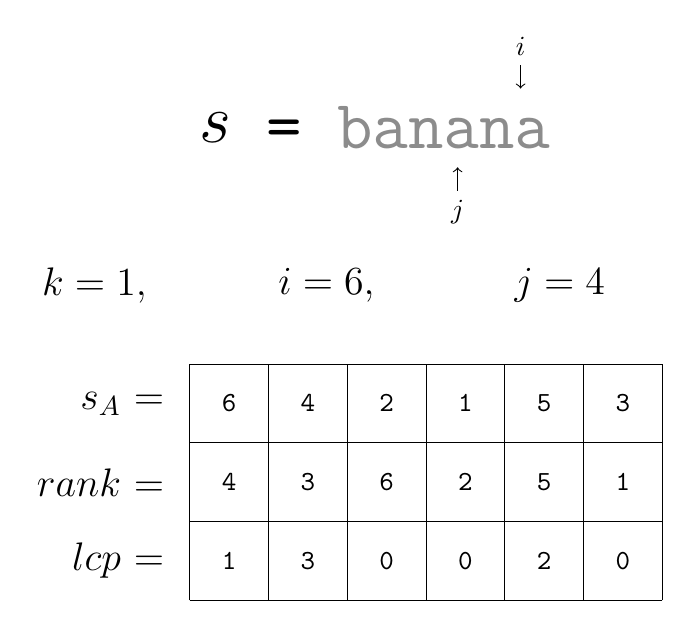
\begin{tikzpicture}
            \node[anchor=west] at (0, 5) { \Huge $s$ };
            \node[anchor=west] at (0.85, 5) { \Huge \texttt{= }\textcolor{gray!90}{\texttt{banana}} };
            \draw[opacity=1,<-] (4.2, 5.5) -- (4.2, 5.8) node[anchor=south] { $i$ };
            \draw[opacity=1,<-] (3.4, 4.5) -- (3.4, 4.2) node[anchor=north] { $j$ };

            \node[anchor=east] at (-0.2, 1.5) { \Large $s_A$ = };
            \draw (0, 1) grid (6, 2);
            \node[anchor=east] at (-0.2, 0.5) { \Large $rank$ = };
            \draw (0, 0) grid (6, 1);
            \node[anchor=east] at (-0.2, -0.5) { \Large $lcp$ = };
            \draw (0, -1) grid (6, 0);

            \node[opacity=1,anchor=west] at (-2.0, 3.0) { \Large $k = 1,$ };
            \node[opacity=1,anchor=west] at (1.0, 3.0) { \Large $i = 6,$ };
            \node[opacity=1,anchor=west] at (4.0, 3.0) { \Large $j = 4$ };

            \node at (0.5, 1.5) { \texttt{6} };
            \node at (1.5, 1.5) { \texttt{4} };
            \node at (2.5, 1.5) { \texttt{2} };
            \node at (3.5, 1.5) { \texttt{1} };
            \node at (4.5, 1.5) { \texttt{5} };
            \node at (5.5, 1.5) { \texttt{3} };

            \node at (0.5, 0.5) { {\texttt{4}} };
            \node at (1.5, 0.5) { {\texttt{3}} };
            \node at (2.5, 0.5) { {\texttt{6}} };
            \node at (3.5, 0.5) { {\texttt{2}} };
            \node at (4.5, 0.5) { {\texttt{5}} };
            \node at (5.5, 0.5) { {\texttt{1}} };

            \node at (0.5, -0.5) { \textbf{\texttt{1}} };
            \node at (1.5, -0.5) { {\texttt{3}} };
            \node at (2.5, -0.5) { {\texttt{0}} };
            \node at (3.5, -0.5) { {\texttt{0}} };
            \node at (4.5, -0.5) { {\texttt{2}} };
            \node at (5.5, -0.5) { {\texttt{0}} };


%            \node at (5.5, 0.5) { \textbf{\texttt{1}} };
        \end{tikzpicture}

    \end{figure}

\end{frame}
